\documentclass[bibtotocnumbered, headsepline,normalheadings,12pt]{report}
\usepackage[utf8x]{inputenc}
\usepackage{ulem}
\usepackage{color}
\usepackage[polutonikogreek,english]{babel}
\usepackage{ucs}
\usepackage{booktabs}
\usepackage{setspace}
\doublespacing
\usepackage{multirow}
\usepackage{listings}
\lstset{basicstyle=\footnotesize\ttfamily,breaklines=true,showstringspaces=false,numbers=left,frame=single,prebreak=\mbox{$\hookleftarrow$}}
\usepackage[hidelinks]{hyperref}
\usepackage[a4paper,margin=2cm]{geometry} 
\usepackage{scrpage}
\usepackage{alltt}
\usepackage{float}
\usepackage{graphicx}
\definecolor{darkblue}{rgb}{0,0,.5}
\hypersetup{pdftex=true, colorlinks=false, breaklinks=true, citecolor=darkblue, linkcolor=darkblue, menucolor=darkblue, pagecolor=darkblue, urlcolor=darkblue,
pdftitle={CACGD 2011 Practical Excercise Report},
pdfauthor={Bartholomäus Dedersen},
bookmarks=true,
bookmarksnumbered=true,
bookmarksopen=true,
bookmarksopenlevel=2}
\usepackage{tabularx}
\pagestyle{headings}
\newcommand{\gdir}%
   {\foreignlanguage{polutonikogreek}}
\usepackage{color}
 \definecolor{light-gray}{gray}{0.80}
\newcommand{\CS}{C\nolinebreak\hspace{-.05em}\raisebox{.6ex}{\scriptsize\bf \#}}

\begin{document}



\begin{titlepage}
\thispagestyle{empty}
 \begin{center}
 \begin{figure}[htbp]
    \centering
     
\includegraphics[width=0.75\textwidth]{fhkiel.png} 
\end{figure}

  \vspace*{2.5cm}
 {\bf \huge CACGD 2011 Practical Exercise Report}
 \vspace*{1cm} \\
 {\Large Game Development\\}
 \vspace{0.5cm}
 {\Large \bfseries Bartholomäus Dedersen\\}
 \vfill
  \vspace*{1.5cm}
\begin{table}[h]
    \centering
    \begin{tabular}{l l}
        Date of Excursion: & Summer 2011 \\ 
        Place: & Iraklion, Crete, Greece \\ 
        Course: & Information Technology \\
        %Date: & 3.1.2013\\
        Date: & \today\\
    \end{tabular}
\end{table}

 \end{center}
\end{titlepage}


\begin{abstract}

    In this report about the practical part of the ``Computational Aspects of Computer Games Development'' programme for two weeks in Crete a
    game programming with the Python programming language is described. The controller is a neural interface for brainwave wavelength reception 
    through three skin-applied electrodes. The game is themed after a fictional Cretan Zombie incursion after the actual event.

\end{abstract}

\tableofcontents \newpage


\chapter{Introduction}
\label{chap:intro}
\gdir{Μετα δέ την του βίου τελευτην ου  μετα ληθης ατιμοι κεῖνται, αλλα μετα μνημης τον αει ξρονον ὑμνοũνται.}\\
-- Xenophon
\vspace{15mm}

This written documentation is a part of the two week conference and tutored exercises in the Cretan state capital Iraklion. The host was the
Technical Educational Institute of Crete, a university with emphasis on applied technology. The conference preparation was done especially through the 
department of Computer Sciences, visible through the timetable.\footnote{Available at \url{https://cacgd2011.teicrete.gr/?q=content/program-lectures}.}.

The author of this work was part of the team from the German Fachhochschule Kiel and reported his personal experience in an formerly online available
diary. This report is supposed to contain the technical description of the proceeding practical lessen from the excursion. Worthwhile to mention 
members of the other college teams were not bound for such task as it functions as an addition to the regular curriculum of the event.
Skills learned should be applied in the resulting game or educational entertainment tool.

Other members of the authors team presented their own results, i.e. a location-based game and a helicopter simulation for children on a mobile platform.

The task was done without the acquired technique of proper software engineering. Instead, a more spontaneous and agile development process was
chosen due to the small team size and new field of work.

The author wants to express his gratitude for having the option to experience Greece and learn new ways of thinking. 

A preceding work from the author is recommended to read as it contains more information in regards to the neural interface, see~\cite{pm}.


\chapter{CACGD Programme}
\label{chap:cacgd}

``Computational Aspects of Computer Game Development'' is part of a series of academic exchanges. Every year until Crete, the 
two week programme was hosted by another European university. Students were housed in the college's respective dormitories and 
supplied with necessary food.

In 2011 on the 11 July, a Monday,  a wide range of educational institutes from Czech, Canada, Great Britain, French, Greece and Germany participated, mostly by
students from Bachelor's courses. The total amount of students was about 70. Half of the audience during the lectures was 
Greek as interested students were invited. Hard-working, responsible organisator from the Greeks George Papadourakis held a
welcome speech and presented the final lecture programme. His own presentation was scheduled at the last day of the 14-day programme.

Instead, George Mamakis held his presentation about ``Visual Perception in Graphic Design – Neuroaesthetics''. Generally spoken, the 
topic evolved about the perception of visual stimuli and how people process and judge them. Especially how feelings are associated 
with pictures. A practical part was the design of a paper sign, capable for using in demonstrations, about the economic crisis. The
authors group solution mainly consisted of a weight scale with weight emphasis money on one side while a house as a sign of material property on 
the other side.
The in-between canteen breaks with associated food description is part of the lost online diary and will not be elaborated in addition to the 
rather mediocre rating giving here.
Second part of the day was filled with George Triantafyllidis' ``The XNA environment for game development''. XNA is used for rapid prototyping of 
computer games and deployment on console based platforms as the XBox from Microsoft or regular Windows machines. It is very interwoven with the
underlaying Dotnet framework and centers around C\# for its main programming language. It has an in-build graphical engine with wrappers for 
Direct3D for acceleration. The idea for rapid development was taken from this lecture for the practical part of this report.

\begin{figure}[H]
    \centering
    
\includegraphics[width=0.6\textwidth]{xna.png}%
    \caption{XNA logo. Source: xblafans.com}
    \label{fig:xna}%
\end{figure}

The next day began with the first non-TEI lecturer Nadine Pasternak from University of La Rochelle in France. His topic, ``Cross-Cultural Communication and Computer Gaming'', was centered about the psychological value of computer games in means of understanding messages from non-native culture origins.
Concluded, gaming can be used to enhance the existing ways of communication between different people and games can be designed to be 
understandable by anyone. The principle of ``easy to learn, hard to master'' was also used on the practical game, similar to chess.

Michel Eboueya, another French lecturer from La Rochelle, presented different ways of graphics in computer games in his ``Computer Graphics In Games Design and For Games''. He showed the way clipping works, i.e. the removal of computational power from processing non-visible graphics to the player. Basics of 
3D design were demonstrated but the lecture was missing practical parts to try out the theory.

On Wednesday ways of ``Data Visualization'' from Nikos Vidakis, a member of the Medialab of the TEI, were shown. As an example figure~\ref{fig:opte}, shows
a simplified graph of various communicating subnets in the Internet. A number of human-selected top level domains are part of the image.
Another explained method were statistics as an educational and entertaining way of presenting game data. Graphs can even represent whole game 
series, e.g. Europa Universalis from Paradox Interactive. The figure~\ref{fig:eu} shows a great example by visualizing the numerical game data into
easier understandable pictures.


\begin{figure}[H]
    \centering
    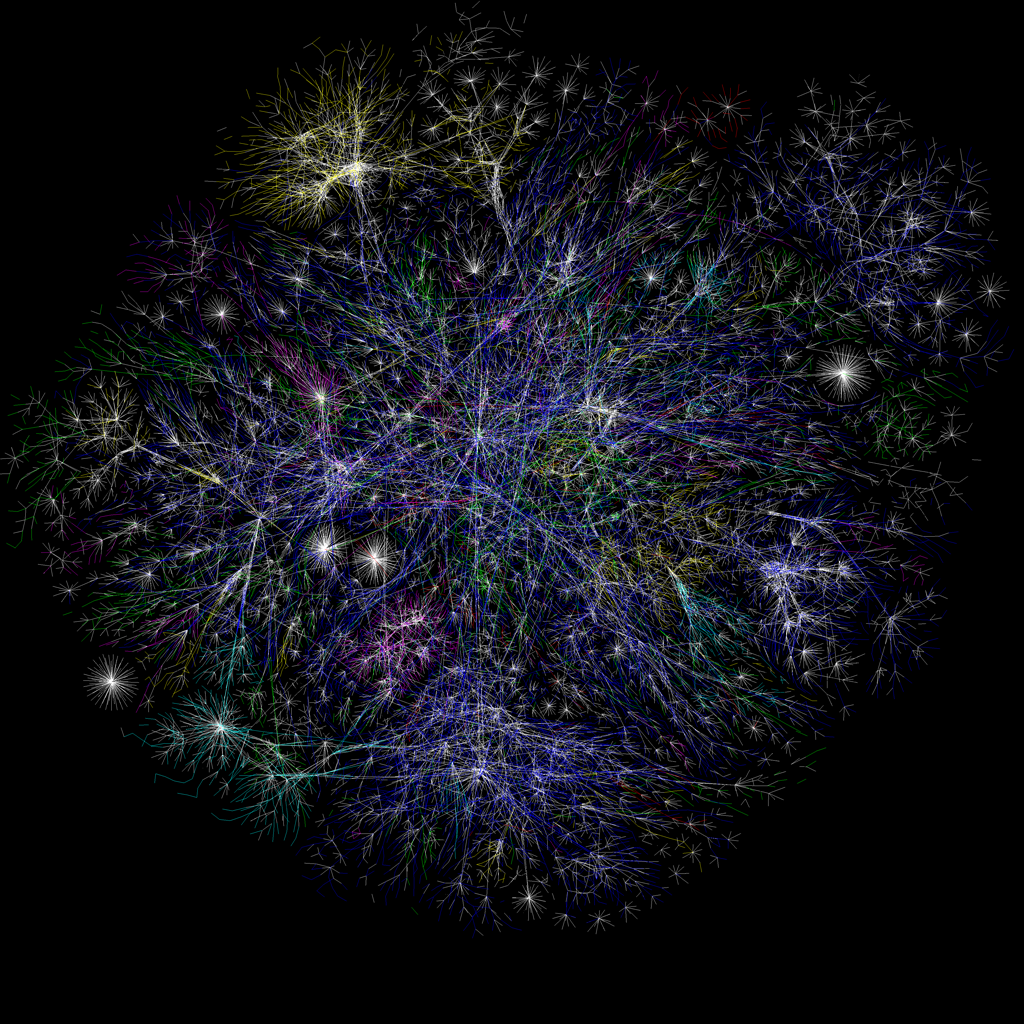
\includegraphics[width=0.6\textwidth]{opte.png}%
    \caption{Visualization of Internet Traffic in Subnets. Source: opte.org}
    \label{fig:opte}%
\end{figure}

\begin{figure}[H]
    \centering
    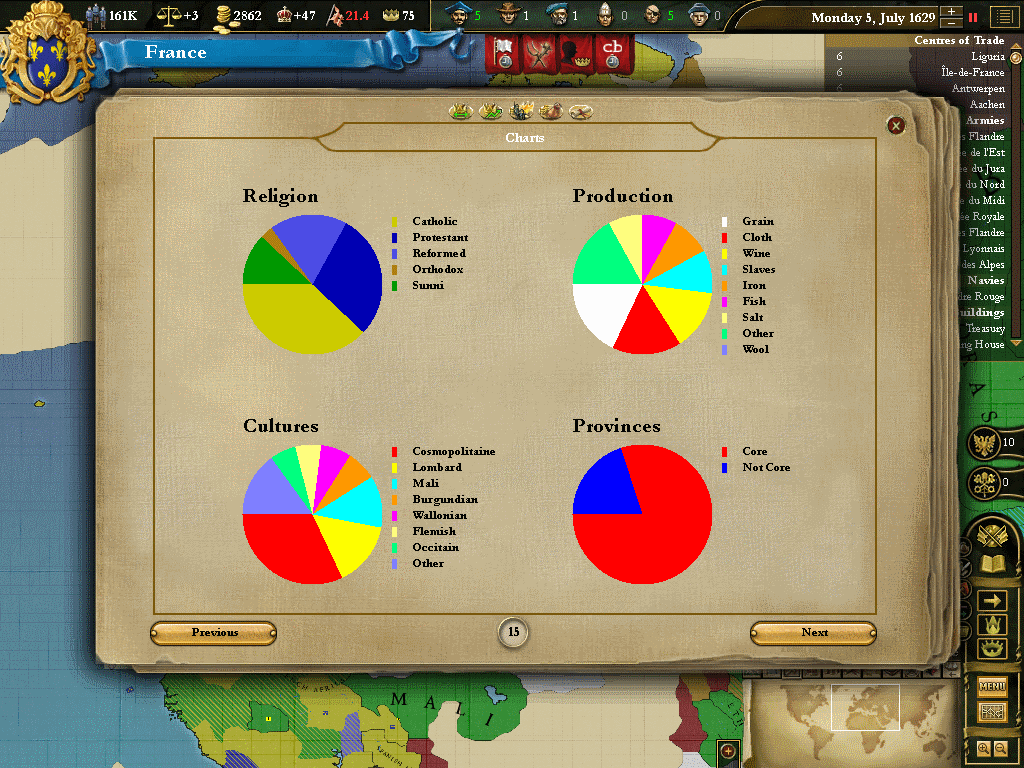
\includegraphics[width=0.6\textwidth]{eu.png}%
    \caption{Europa Universalis 3 as example for data-centric games. Source: paradoxplaza.com}
    \label{fig:eu}%
\end{figure}

After the lunch the highly anticipated ``Security Issues in Computer Games'' by TEI's Harry Manifavas showed the listeners how in-game payments are 
procured and how real money can be lost in such games. The economics of virtual currencies in games like Linden Dollars in Second Life are similar
to real-world currencies, including fluctuation and speculation. As an example, the worth of Bitcoins, the virtual and completely based in computing power,
not in trust, is shown in figure~\ref{fig:bc}. The total availability of bitcoins is limited by the total calculation of a specific hash function as further
explained in~\cite{bitcoin}. The ability to forge such transaction is limited to the extend the attacker can provide a higher amount of computation power 
compared to the whole distributed Bitcoin network.

\begin{figure}[H]
    \centering
    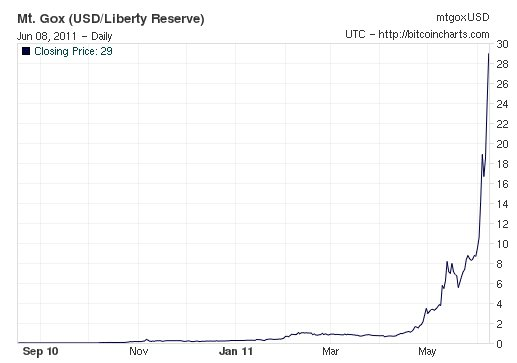
\includegraphics[width=0.6\textwidth]{bc.jpg}%
    \caption{Bitcoin to USD exchange rates. Source: bitcoincharts.com}
    \label{fig:bc}%
\end{figure}

Thursday was the day of neuronal networks and artificial intelligence. In the morning, Ali Ghorbani from the University of New Brunswick in Canada was 
giving a speech about ``Unsupervised Learning''. He gave a firm introduction to artificial learning with Hebbian networks as to

\[ w_{ij} = \frac{1}{p} \sum_{k=1}^p x_i^k x_j^k\]

where the connection between the neurons \(x_i\) and \(x_j\) is used to calculate the weight \( w \). It goes summed over generations called \( k \) in \( p \) 
training patterns. The formula simulates the learning in the simplified weight value for finding patterns in large input datasets. Similar learning is 
applied in the practical exercise in addition to a factor which weights the different wavelengths according to their physical reaction.
The opposite of supervised learning where a target value is precalculated or given by a human so the weights can be adjusted.


In the afternoon, Claude Frasson from the University of Montral in Canada had a talk
about ``Intelligent Tutoring Systems''. The topic evolved around educational systems for teaching support. Mainly projects for highschool teaching 
were shown.

The last day of the week was introduced by the British archeologist Gareth Owens. His talk about his DVD project about Cretan ancient history 
was dominated by his enthusiasm for the Phaistos disk. The multimedia effects of the DVD have video snippets combined with interactive moving sprites, 
simulating an excavation. Sound effects encapsulate the educational content in a game-like immersion. Practical part of the lesson was a discussion about
the possible meaning of the yet unknown content of the writing on the disk as shown in figure~\ref{fig:pha}. The vocal intonation is known but the 
meaning of the context and even words of the used language Linear A. The current hypothesis of Gareth Owens concerning the face symbol with 
spiked hair is the connected with the meaning of ``mother''.


\begin{figure}[H]
    \centering
    
\includegraphics[width=0.8\textwidth]{pha.png}%
    \caption{Front of the Phaistos Disk. Source: couk.com}
    \label{fig:pha}%
\end{figure}

The afternoon lecture was also held by Mr Owens and were focused around the Minoan history of Crete. Strabo writes about Crete that it ``flourished from the 
excellence of the soil, which is peculiarly adapted for breeding horses, and the growth of fine crops.'' in his \gdir{Γεωγραφικά}. Minoans lived 
before him on the island from roughly 2500 to 1500 BC and represented native inhabitants of Greece, so called Pelasgians. Strabo says ``that the Pelasgians had been a great people can be documented also by other sources. Namely, Menecratos Elaita, tells us in his book about the origins of the cities that the entire maritime region which now is called Ionia, starting from Mycale and the neighboring islands, has formed once the dwellings of the Pelasgians.''

First appearance of agriculture in Europe coming from the Middle East is linked to Crete as well as the mythological tale of the Minotaurus. Moreover, 
a relation to the Argonauts which searched for the Golden Fleece under the hero Jason could be established as ancient Crete was a hub for trading and 
was renowned with its riches in gold. Their ship, the Argo, is supposed to be buried on Crete.

Basic mythology was needed as the weekend's excursion lead the students to the archeological site of Knossos. It was the ancient ruling palace of the Minoan
king with a combined grain storage. The food was collected by the king and guarded for asserting power over the peasants and secure emergency ratios for 
upcoming droughts. Sophisticated inventions as a non-electric climatization were found on the excavation site. Cold air from the sun overcast hill towards
the coast went through internal wind canals to the top floors of the palace.

``Survey on Game AI theory and Algorithms'' on the next week's Monday was held by George Mamakis were the link was explained to his first lecture about
the effects of graphics. Students were animated to develop their own game formulas. George Bebis from the University of Nevada in USA showed medical 
usage of computer vision and showed his research lab with a short introduction to his scientific area. Image processing is also used in games for collision 
detection. Moreover, prototyped hardware for automatic traffic measurement of was shown.

\begin{figure}[H]
    \centering
    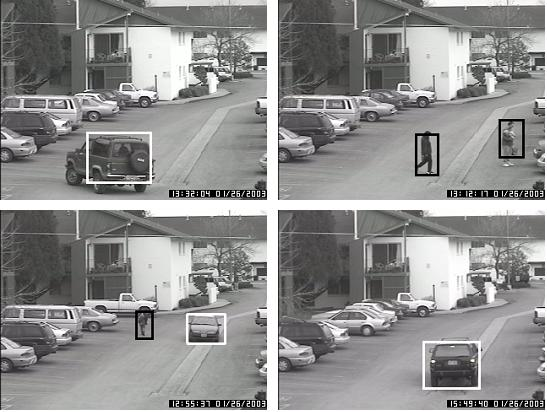
\includegraphics[width=0.8\textwidth]{bebis.jpg}%
    \caption{Traffic Detection and Analysis. Source: cse.unr.edu}
    \label{fig:bebis}%
\end{figure}

Next day's morning started with a lecture about game ethics by the British lecturer Paul Javis from the University of Glamorgan. Problematic questions as 
how to depict gore and violence and other questionable but realistic content is shown by example in games. The students were split in different groups which 
had to prepare and present arguments of one side for a specific question. Later on, the results were presented in a talkshow-like discussion with two 
groups arguing and the other students watching and judging about the \textsl{ethically right} position. As Zombies are ethically accepted when the 
violence level is kept under a certain culturally dependent threshold which is aimed for in the practical part only a minor part could be used.

``Principles of Artificial Intelligence'' from Andrew Ware from the same university as the previous speaker gave a general introduction to artificial learning 
and tried to show examples of Non-Player character behaviour in current games. The limitations of a complete simulation in regards to computational resources
were explained in a slide show.
Wednesday continued the speaks of the previous days.

Michal Hradiš from Brno University of Czech Republic introduced new methods for interaction in games in his talk. The author of this work got his 
inspiration by the man-machine interface from this lecturer. 3D glasses and other gear was also part of Thursday's morning.

\begin{figure}[H]
    \centering
    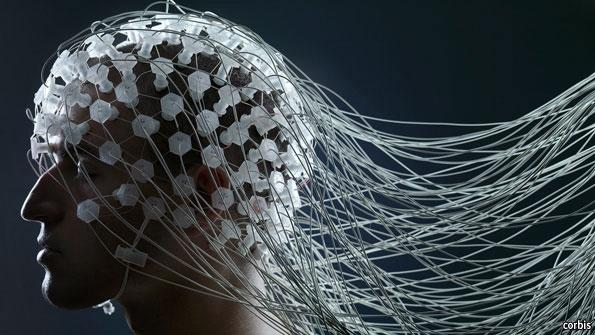
\includegraphics[width=0.6\textwidth]{eeg.png}%
    \caption{Futuristic EEG Device. Source: digitaltrends.com}
    \label{fig:bebis}%
\end{figure}

The second half of the day was succeeded by the same lecturer where he presented more real-world practical smart home implementations of entertainment. 
Augmented reality as an addition to the typical game experience was discussed and how such devices could alter the communication structure of the society.

On the last day of the games programme Helmut Dispert\footnote{Supposedly one, if not the only, reader of this document.} gave an overview of 
Ambient Intelligence. The author of this work wrote numerous exams and reports about this topic and was the main \xout{claquer} critique listener.  
The topic was a general introduction to the idea of ubiquitous computing, available devices on the market and location based services.

George Papadourakis held the final presentation about Quake 3 and general first person shooters. Mainly, the final certificates were handed out 
with a special souvenir from Crete.


\chapter{Game Idea}
\label{chap:idea}

background story:
zombie attack on crete
Graveyard inspired by Rethymno
phaistos disk is the source of zombiism

zombies and easy understandable games on rise
other similar games


\chapter{Framework}
\label{chap:framework}

pygame
neuronal network
pyserial

\chapter{Implementation}
\label{chap:impl}

code

demo

\chapter{Evaluation}
\label{chap:eva}

calibration time
learning algorithms

\chapter{Summary}
\label{chap:sum}

\nocite{*}
\bibliographystyle{acm}
\bibliography{common}
\listoffigures
\lstlistoflistings
\begingroup \let\clearpage\relax
\listoftables \endgroup

\end{document} 
